\scanpage{49}
\inserted{$\Delta_{n+2}(0,1,c_0,\ldots,c_{n-1})$}
\[
\begin{aligned}
\deleted{\unsure{\det}}\ \Delta_n(\underbrace{c_0,\ldots,c_{n-1}}_{n\ \text{arg.}})
&=\unsure{-|{}}\det\left(\begin{array}{cccccccc}
0&-1&0&0&0&0&\cdots&0\\
-1&2&-c_0&0&0&0&\cdots&0\\
0&-c_0&2c_0&-c_1&0&0&\cdots&\vdots\\
0&0&-c_1&2c_1&-c_2&0&\cdots&\vdots\\
0&0&0&&\ddots&-c_3&&0\\
\vdots&\vdots&\vdots&&&&&-c_{n-1}\\
0&0&0&\text{--}&\text{--}&0&-c_{n-1}&2c_{n-1}
\end{array}\right)_{\leftarrow(\text{ordre }n+2)}\\
&=\det\left(\begin{array}{ccccccc}
2c_0&-c_1&0&0&0&\text{---}&0\\
-c_1&2c_1&-c_2&0&0&&\\
0&-c_2&2c_2&-c_3&0&\cdots&\\
0&0&-c_3&2c_3&-c_4&&\vdots\\
\text{--}&\text{--}&\text{--}&\text{--}&\text{---}&\text{--}&-c_{n-1}\\
0&0&0&0&\cdots\ 0&-c_{n-1}&2c_{n-1}
\end{array}\right)_{\leftarrow\,\text{ordre }n}
\end{aligned}
\]

\[
\boxed{\Delta_n(c_0,\ldots,c_{n-1})=2c_0\Delta_{n-1}(c_1,\ldots,c_{n-1})\unsure{-|+}c_1^2\Delta_{n-2}(c_2,\ldots,c_{n-1})}
\]

\[
\Delta'_n(c_0,\ldots,c_{n-1})=
\begin{cases}
\Delta_n(c_0,\ldots,c_{n-1})&\text{si $n$ \deleted{\unsure{im}}pair}\\
\frac12\Delta_n(c_0,\ldots,c_{n-1})&\text{si $n$ impair}
\end{cases}
\]

Posons
\[
\left.\begin{aligned}
c_0&=\beta_0,\ \unsure{c}\\
c_1&=\beta_0\beta_1\\
&\ldots\\
c_{n-1}&=\beta_0\beta_1\ldots\beta_{n-1}
\end{aligned}\right\}\quad n\!-\!1\ \text{arguments }\beta_i
\]

\[
\begin{aligned}
\delta_n(\beta_0,\ldots,\beta_{n-1})&=\Delta_n(\beta_0,\beta_0\beta_1,\ldots,\beta_0\beta_1\ldots\beta_{n-1})\\
\delta'_n(\beta_0,\ldots,\beta_{n-1})&=\Delta'_n(\ldots)=\begin{cases}
\delta_n(\beta_0,\ldots,\beta_{n-1})&n\ \text{\unsure{pair}}\\
\frac12\delta_n(\beta_0,\ldots,\beta_{n-1})&n\ \text{impair}
\end{cases}
\end{aligned}
\]

\[
\begin{aligned}
\Delta_n,\Delta'_n,\deleted{\unsure{\Delta'_n|\overline{\Delta'_n}}}\inserted{\widetilde{\Delta}'_{\unsure{n|j}}}&\in\mathbb Z[C_0,\ldots,C_{n-1}]\\
\delta_n,\delta'_n,\widetilde{\delta}'_n&\in\mathbb Z[B_0,\ldots,B_{n-1}]\\
\Delta'_n[C_0,\ldots,C_{n-1}]&=C_{n-1}\widetilde{\Delta}'_{\unsure{n-1|n}}(C_0,\ldots,C_{n-1})\\
\delta'_n[B_0,\ldots,B_{n-1}]&=B_{n-1}\widetilde{\delta}'_n(B_0,\ldots,B_{n-1})
\end{aligned}
\]

\[
\begin{aligned}
\Delta_1(c_0)&=2c_0,\quad\Delta'_1(c_0)=c_0\quad\widetilde{\Delta}'_1(c_0)=1\\
\Delta_2(c_0,c_1)&=4c_0c_1-c_1^2=c_1(4c_0-c_1)\quad\widetilde{\Delta}'_2(c_0,c_1)=4c_0-c_1)\\
\Delta_3(c_0,c_1,c_2)&=2c_2(4c_0c_1-c_0c_2-c_1^2),\quad
\Delta'_3=\deleted{2}c_2(4c_0c_1-c_0c_2-c_1^2),\\
&\ldots\qquad\inserted{\widetilde{\Delta}'_3(c_0,c_1,c_2)=4c_0c_1-c_0c_2-c_1^2}
\end{aligned}
\]

\margin{chgt notation}\margin{\unsure{mon signe|sous-signe|en} des \unsure{lignes|signes|origine} des paires}
\[
\begin{aligned}
\Delta_n(C_0,\ldots,C_{n-1})={}&\sum_{0\le p\le[n/2]}(-1)^p2^{n-2p}\sum_{\substack{\text{suites de }p\\\deleted{\unsure{\text{intervalles de}}}\\\text{él. de }\mathcal P_2([0,n-1])\\\text{disjoints}\\
\deleted{\unsure{K}}\,J_1\ldots J_p,\ \deleted{\unsure{\text{à deux él.}}}}}
\prod_{i\in J'}C_i\prod_{j\in J''}C_j^2
\end{aligned}
\]
$J=\bigcup_{1\le i\le p}J_i$ \quad $J'=[0,n-1]\setminus J$ \quad $J''=$ ens des derniers éléments des $J_i$ $(J''\in\mathcal P_p([0,n-1]))$

\margin{\uline{NB} Il n'y a pas de \unsure{cancell.tion|cancell.|cancellation} de termes}

\deleted{$\unsure{\Delta_n(C_0,\ldots,C_{n-1})}=$} Le monôme $M=\prod_{i\in J'}C_i\prod_{j\in J''}C_j^2$ s'écrit aussi

\[
\begin{aligned}
&\deleted{F_n(c_1,\ldots,c_n)=\beta_0}\\
&B_0^n B_1^{n-1+\varepsilon_2}B_{\unsure{3|2}}^{n-2+\varepsilon_3}\ldots B_{n-1}^{\varepsilon_n}
\qquad\varepsilon_k\in\{0,1\}\qquad2\le k\le n\\
&\varepsilon_k=1\ \text{sss }\ k\in J'''\quad\text{(il y \deleted{\unsure{en}} a $p$ tels $k$)}
\end{aligned}
\]

\figure{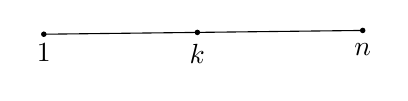
\begin{tikzpicture}[x=.75cm,y=.6cm]
\draw (0,0)--(5.4,.08);
\foreach \x/\lab in {0/1,2.6/k,5.4/n}{\fill (\x,.08*\x/5.4) circle(1pt);\node[below] at (\x,0) {$\lab$};}
\end{tikzpicture}}

\[
M=\prod_{1\le i\le n}C'_i\qquad
C'_i=\begin{cases}
C_i&\text{si }i\in J'\\
C_j&\text{si }j\in J''\\
C_{j+1}&\text{si }j\in\unsure{\complement J'|\complement J''}\ \unsure{J''}
\end{cases}
\]

\[
\begin{aligned}
\delta_n(B_0,\ldots,B_{n})&=
 B_0^n B_1^{n-1}\ldots B_{n-1}^{1}\underbrace{L_n(B_1,\ldots,B_{n-1})}_{\text{polynôme \deleted{\unsure{homogène de degré $[n/2]$}}}}
 \deleted{\unsure{\text{degré}}}
\end{aligned}
\]
\margin{Attention, \unsure{pas 0|$p\to0$|$p\geq0$}!} $C'_i$ contient en facteur $B_k$ \deleted{\unsure{(et ce facteur}} à la puiss. 1 exactement) sss \deleted{\unsure{entier}} $i\ge k$, \uline{ou} $i=k-1$ \uline{et} $i\in J^{\unsure{'''|''}}$ i.e. $k\in J''$

\[
\begin{aligned}
L_n(B_1,\ldots,B_{n-1})
&=\sum_{0\le p\le[n/2]}(-1)^p2^{n-2p}
\sum_{\substack{\deleted{\unsure{\text{suites de }p\,J_i}}\\J\in\mathcal P_p([1,n-1])\\J\text{ ne contient pas 2}\\\text{entiers consécutifs}}} B_J\\
&=2^n\unsure{-|+}2^{n-2}\sum_{\unsure{1|0}\le i\le n-1}B_i
+2^{n-4}\sum_{\substack{1\le i<j\le n-1\\j\ne i+1}}B_iB_j\\
&\quad-2^{n-6}\sum_{\substack{1\le i<j<k\le n\\\vdots\quad\vdots}}B_iB_jB_k+\ldots
\end{aligned}
\]
\margin{\unsure{Attention|les}, \unsure{$n-1$ et non $n$|non circulaire} !}
% archive sheet number: 48
